\documentclass[frenchb]{article}
\usepackage[utf8]{inputenc}

\usepackage{graphicx}
\usepackage{color}

\usepackage{geometry}
\geometry{hmargin=2.5cm,vmargin=1.5cm}


\usepackage[T1]{fontenc}
\usepackage{a4wide}
\usepackage{graphicx}
\usepackage{amssymb}
\usepackage{amsmath}
\usepackage{color}
\usepackage{babel}
\usepackage{mathtools}

\usepackage{float}
\restylefloat{table}


\begin{document}

\begin{figure}[t]
\centering

\includegraphics[width=5cm]{inp_n7.png}
\end{figure}

\title{\vspace{4cm} \textbf{Études de chaînes de transmission sur fréquence porteuse}}
\author{Nom des auteurs\\ \textsc{Cazes} Noa\\ \textsc{Martin} Cédric}
\date{\vspace{11cm} Département Sciences du Numérique - Première année \\
2019-2020 }

\maketitle

\newpage
\tableofcontents
\listoffigures

\newpage


\section{Introduction}

\setlength\parindent{0.5cm}
Après avoir étudié les chaînes de transmisssion en bande de base, notre étude se porte ici sur les chaînes de transmission sur fréquence porteuse. Il n'est plus alors question d'étuder l'impact des filtres de réception ou de mise en forme sur l'efficacité spectrale et en puissance, mais plutôt de comparer chaîne sur fréquence porteuse et sa chaîne passe-bas équivalente, puis de comparer l'impact du mapping sur l'efficacité spectrale et en puissance.  


\section{Utilisation de la chaine passe-bas équivalente pour le calcul et l'estimation du taux d'erreur binaire}

L'objectif de cette partie est de montrer que le taux d'erreur binaire obtenu pour une transmission est identique que l'on implante la chaine de transmission sur fréquence porteuse ou bien la chaine passe-bas équivalente. L'étude sera réalisée pour une transmission QPSK.

\subsection{Etude théorique}
On considère la chaine de transmission passe-bas équivalente à une chaine de transmission QPSK (symboles $d_k \in \left\{\pm 1 \pm j\right\}$), avec filtre de mise en forme et filtre de réception en racine de cosinus surélevé de même roll off et un canal à bruit additif blanc et Gaussien. La figure \ref{rcf} donne le tracé de la réponse en fréquence globale de la chaine de transmission : $G(f)=H(f)H_r(f)$, où $H(f)$ représente la réponse en fréquence du filtre de mise en forme et $H_r(f)$ la réponse en fréquence du filtre de réception.

\begin{figure*}[h!]
\begin{center}
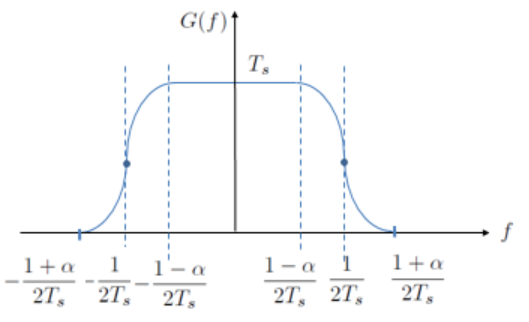
\includegraphics[width=7cm]{RCF.PNG}
\end{center}
\caption{Réponse en fréquence de la chaine de transmission} \label{rcf}
\end{figure*}

\begin{enumerate}
    \item Calculer l'énergie symbole $E_s$ à l'entrée du récepteur. Attention $E_s$ représente la véritable énergie reçue, c'est-à-dire qu'elle doit être calculée à partir de la véritable puissance du signal reçu, pas à partir de celle de l'enveloppe complexe associée.
	\begin{equation*}
	\begin{split}
	P &= \int_\mathbb{R}S_x(f) \ \mathrm{d}f \\
	P &= \frac{1}{2} \int_\mathbb{R}S_{x_e}(f) \ \mathrm{d}f \\
    \end{split}
   \end{equation*}
   
   Sachant que : 
   $$ m_d = 0 $$
   $$ \sigma_d^2 = 1 $$
   
   D'où : 
   \begin{equation*}
	\begin{split}
	P &= \frac{1}{2} \int_\mathbb{R}S_{x_e}(f) \ \mathrm{d}f \\
	P & = \frac{1}{2T_s} \int_\mathbb{R}|G(f)| \ \mathrm{d}f \\
	P & = \frac{1}{2T_s} \int_{\frac{-(1+\alpha)}{2 T_s}}{\frac{-(1+\alpha)}{2 T_s}} |G(f)| \ \mathrm{d}f \\
	P & = \frac{1}{2T_s}
    \end{split}
   \end{equation*}
   En effet, 
   $$ \int_{\frac{-(1+\alpha)}{2 T_s}}^{\frac{-(1+\alpha)}{2 T_s}} |G(f)| \ \mathrm{d}f = 1 $$
   
   En conclusion : 
   $$\boxed{E_s = \frac{1}{2}}$$
        
        

    
    \item Calculer la puissance du bruit sur chaque voie (I et Q) en sortie du filtre de réception.
    $$ n_e(t) = n_I(t) + j n_Q(t) $$
    Soit $n(t)$ le bruit calculé précédemment pour des chaînes en bande de base. 
    
    \begin{equation*}
    \begin{split}
    S_{n_e(f)} & = 4 S_n(f+f_p) U(f+f_p) \\
    S_{n_e(f)} & = 4 \text{x} \frac{N_0}{2} \text{x} 1 \\
    S_{n_e(f)} & = 2 N_0 \\
    \end{split}
    \end{equation*}
    
    Comme : 
    $$ S_{n_I}(f) = S_{n_Q}(f) $$
    
    \begin{equation*}
    \begin{split}
    S_{n_e(f)} & = |N_e(f)|^2 \\
    S_{n_e(f)} & = |N_I(f)|^2 + |N_Q(f)|^2\\
    S_{n_e(f)} & = 2 \ |N_I(f)|^2 \\
    \sigma_I^2 & = \sigma_Q^2(f) = N_0 \\
    \end{split}
    \end{equation*}
    
    \item Les deux voies I et Q étant indépendantes, donner le taux d'erreur symbole de la modulation QPSK en fonction de ceux des voies I et Q ($TES_I$ et $TES_Q$).
    \begin{equation*}
    \begin{split}
    TES & = \mathbb{P}(\hat{d}_m \ne d_m) \\
    & = \sum_{m} \mathbb{P}(\hat{d}_m \ne d_m) \\
    & = \sum_{m} \mathbb{P}(\hat{a}_m \ne a_m) + \sum_{m} \mathbb{P}(\hat{b}_m \ne b_m) - \sum_{m} \mathbb{P}(\hat{a}_m \ne a_m) \sum_{m} \mathbb{P}(\hat{b}_m \ne b_m)\\ \text{D'après l'indépendance des deux voies.}
    \end{split}
    \end{equation*}
           
    \item En suppposant les termes du deuxième ordre négligeables ($TES_I \times TES_Q \sim 0$) , donner le taux d'erreur symbole de la modulation QPSK en fonction de $TES_I$ uniquement.
    
    On a : 
    $$ TES = TES_I + TES_Q - TES_I \times TES_Q $$
    Comme : 
    $$TES_I \times TES_Q \sim 0$$
    On a : 
    $$\boxed{TES = 2 TES_I}$$
    
    \item Déterminer $TES_I$ en fonction de $\frac{E_s}{N_0}$, $E_s$ correspondant à la véritable énergie reçue. On supposera que les instants d'échantillonnage et l'organe de décision sont optimaux.
    
    \begin{equation*}
    \begin{split}
    TES & = \mathbb{P}(\hat{d}_m \ne d_m) \\
    & = 2 \sum_{m} \mathbb{P}(\hat{a}_m \ne a_m) \\
    & = 2 \left[\mathbb{P}(a_m = -V) \ \mathbb{P}(\hat{a}_m = + V | a_m = -V) + \mathbb{P}(a_m = +V) \ \mathbb{P}(\hat{a}_m = - V | a_m = +V)\right] \\
    & = \mathbb{P}\left(z_m \geq 0 \ | \ z_m = -V g(t0) + \omega_m\right) + \mathbb{P}\left(z_m \leq 0 \ | \ z_m = V g(t0) + \omega_m\right)\\
    & = \mathbb{P}\left(\frac{\omega_m}{\sigma} \geq \frac{Vg(t0)}{\sigma}\right) + \mathbb{P}\left(\frac{\omega_m}{\sigma} \leq \frac{-Vg(t0)}{\sigma}\right)\\
    & = 2 \mathbb{P}\left(\frac{\omega_m}{\sigma} \geq \frac{Vg(t0)}{\sigma}\right) \\
    & = 2 Q\left(\frac{V g(t_0)}{\sigma} \right) \\
    \end{split}    
    \end{equation*}
         
        D'après la définition de la puissance du bruit:
        
        \begin{equation*}
        \begin{split}
        P_{\omega} &= \int_\mathbb{R}S_{\omega}(f) \ \mathrm{d}f \\
        \end{split}
        \end{equation*}
        
        D'après la formule de Wiener-Lee:
        
        \begin{equation*}
        \begin{split}
        P_{\omega} = \int_{\mathbb{R}}|H_r(f)|^2 \frac{N_0}{2} \ \mathrm{d}f \\
        \end{split}
        \end{equation*}
        
        D'après notamment l'égalité de Parseval, on en déduit:
        \begin{equation*}
        \begin{split}
        \sigma^2 &= \frac{N_0}{2}  \\
        \sigma &= \sqrt{\frac{N_0}{2}} \\
        \end{split}
        \end{equation*}
        
        Avec : 
        \begin{equation*}
        \begin{split}
        V = 1 \\
        g(t0) = \frac{1}{2}\\
        E_s = \frac{1}{2} \\
        \end{split}
        \end{equation*}
        On a :
        \begin{equation*}
        \begin{split}
        \frac{V g(t_0)}{\sigma} = \frac{E_s}{N_0} \\
        \end{split}
        \end{equation*}
        
        Donc :
        \begin{equation*}
        \begin{split}
        TES = 2 \ Q\left(\sqrt{\frac{E_s}{N_0}} \right) \\
    	    \end{split}
        \end{equation*} 
        
        Or les deux voies sont indépendantes, donc : 
        $$ \boxed{TES_I = TES_Q =  Q\left(\sqrt{\frac{E_s}{N_0}} \right)} $$
    \item En déduire le taux d'erreur binaire de la chaine de transmission QPSK en fonction de $\frac{E_b}{N_0}$.
    
    Avec un mapping de Gray, 
    \begin{equation*}
    \begin{split}
    	     nb_{symboles faux} & \simeq nb_{bits faux} \\
         TES & \simeq TEB \ log2(M)\\
         TES & \simeq 2 TEB\\
         TEB & \simeq \frac{1}{2} TES \\                 
         TEB & \simeq Q\left(\sqrt{\frac{E_s}{N_0}}\right) \\      
     \end{split}
     \end{equation*}
\end{enumerate}


\subsection{Implantation sous Matlab}
\subsubsection{Implantation de la chaine sur fréquence porteuse}
\begin{enumerate}
    \item Tracer les signaux générés sur les voies en phase et en quadrature ainsi que le signal transmis sur fréquence porteuse.
    \par\leavevmode\par
    \setlength\parindent{0.5cm}
    Les figures \ref{F11} et \ref{F111} représentent respectivement  les signaux générés sur les voies en phase et en quadrature, et la figure \ref{F12} représente le signal transmis sur fréquence porteuse. 
    \begin{figure}[ht!]
    		\centering
		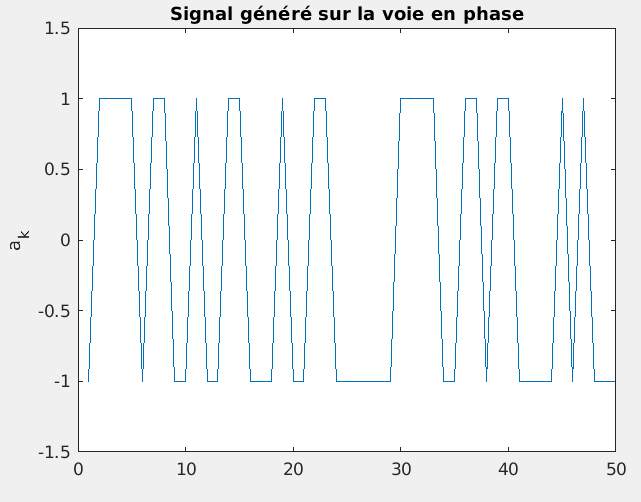
\includegraphics[width=10cm]{C1phase.png}	              	 	\caption{Signaux générés sur la voie en phase. \label{F11}}
	\end{figure}
	
	\begin{figure}[ht!]
    		\centering
		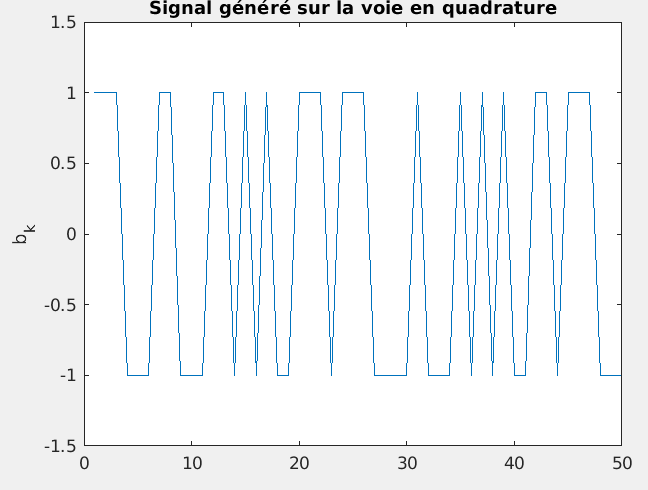
\includegraphics[width=10cm]{C1quadra.png}	              	 	\caption{Signaux générés sur la voies en quadrature. \label{F111}}
	\end{figure}
	
	\begin{figure}[ht!]
    		\centering
		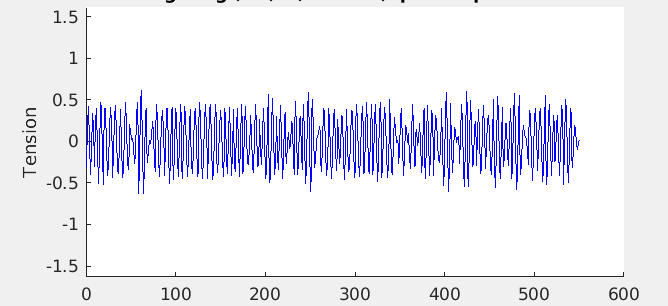
\includegraphics[width=10cm]{C1signal.png}		              	 	\caption{Signal transmis sur fréquence porteuse. \label{F12}}
	\end{figure}
	
    \item Estimer par périodogramme puis tracer la densité spectrale de puissance du signal modulé sur fréquence porteuse. Le tracé observé (forme, position) correspond-il à ce qui est attendu en théorie ? Expliquez votre réponse.
    \par\leavevmode\par
    \setlength\parindent{0.5cm}
    La figure \ref{F13} représente l'estimation la densité spectrale de puissance du signal modulé sur fréquence porteuse. 
    \begin{figure}[ht!]
    		\centering
		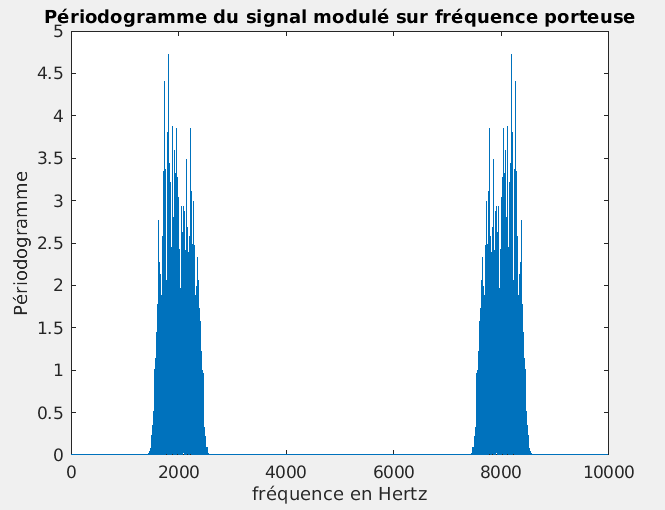
\includegraphics[width=10cm]{C1perio.png}		              	 	\caption{DSP du signal modulé sur fréquence porteuse. \label{F13}}
	\end{figure}
    \newpage
    Ce qui est attendu est la répétition de la DSP du signal non modulé sur fréquence porteuse, l'une centrée sur $f_p$ et l'autre centrée sur $-f_p$. 
    
    La DSP du signal non modulé sur fréquence porteuse est celui d'un signal tronqué temporellement, ce qui induit une périodisation fréquentielle du signal (de fréquence $F_e$), donc les courbes présentes en $f_p$ et $-f_p$, devraient être présentes entre $0$ et $F_e$, en $F_e-f_p = 8000 Hz$ et en $fp_ = 2000 Hz$. 
    
	Ce qui est bien le cas ici. 
    \item Implanter la chaine complète sans bruit afin de vérifier que le TEB obtenu est bien nul.
    \par\leavevmode\par
    \setlength\parindent{0.5cm}
    Le TEB obtenu est bien nul.
    
    \item Rajouter le bruit et tracer le taux d'erreur binaire obtenu en fonction du rapport signal à bruit par bit à l'entrée du récepteur ($E_b/N_0$) en décibels. On prendra des valeurs de $\left(E_b/N_0\right)_{dB}$ allant de $0$ à $6$ dB.
    \par\leavevmode\par
    \setlength\parindent{0.5cm}
    La figure \ref{F14} représente le taux d'erreur binaire obtenu en fonction du rapport signal à bruit par bit à l'entrée du récepteur ($E_b/N_0$) en décibels.
    \begin{figure}[ht!]
    		\centering
		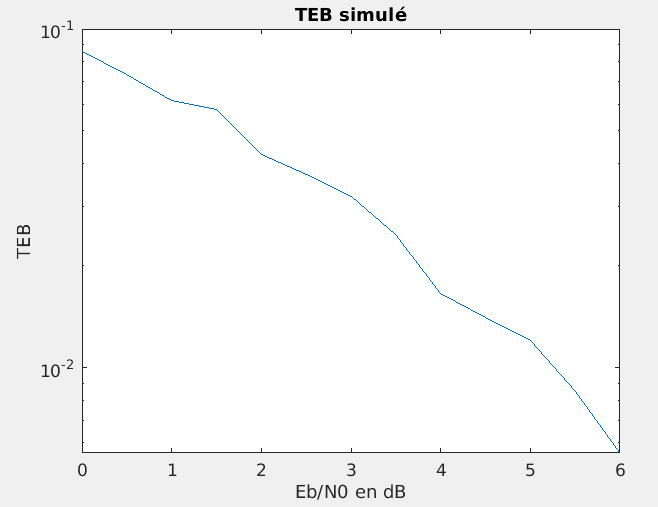
\includegraphics[width=10cm]{C1tebs.png}		              	 	\caption{TEB en fonction de $\left(E_b/N_0\right)_{dB}$. \label{F14}}
	\end{figure}
    \newpage
    \item Comparer le TEB simulé au TEB théorique de la chaine étudiée (tracé superposés sur une même figure). Ce tracé doit permettre de valider le bon fonctionnement de votre chaine de transmission.
     \par\leavevmode\par
    \setlength\parindent{0.5cm}
    La figure \ref{F15} représente la comparaison entre le TEB simulé et le TEB théorique de la chaine étudiée en fonction du rapport signal à bruit par bit à l'entrée du récepteur ($E_b/N_0$) en décibels.
    \begin{figure}[ht!]
    		\centering
		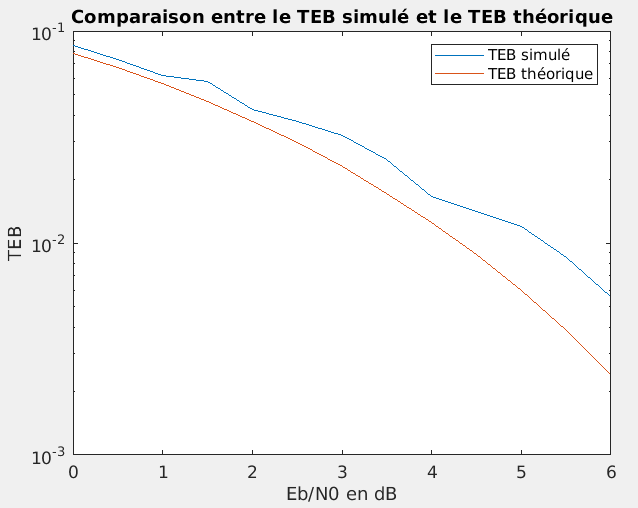
\includegraphics[width=10cm]{C1teb.png}		              	 	\caption{TEB simulé et TEB théorique en fonction de $\left(E_b/N_0\right)_{dB}$. \label{F15}}
	\end{figure}
	
	Les courbes sont sensiblement les mêmes, cela permet de valider le bon fonctionnement de notre chaine de transmission
\end{enumerate}

\subsubsection{Implantation de la chaine passe-bas équivalente}
\begin{enumerate}
    \item Tracer les signaux générés sur les voies en phase et en quadrature.
    
    \par\leavevmode\par
    \setlength\parindent{0.5cm}
    Les figures \ref{F21} et \ref{F211} représentent respectivement  les signaux générés sur les voies en phase et en quadrature. 
    \begin{figure}[ht!]
    		\centering
		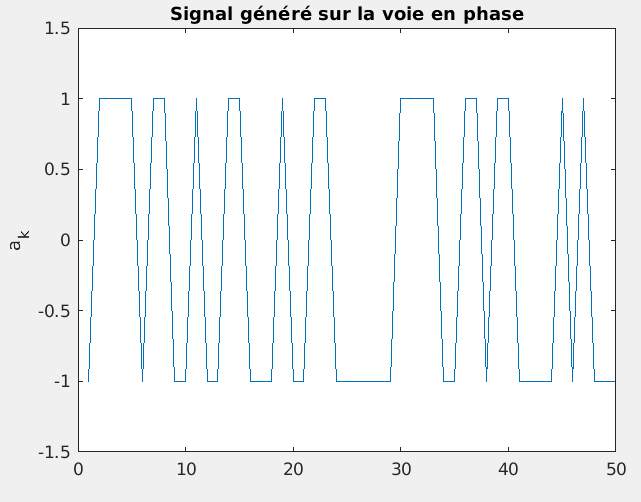
\includegraphics[width=10cm]{C1phase.png}	              	 	\caption{Signaux générés sur la voie en phase (chaîne équivalente passe-bas). \label{F21}}
	\end{figure}
	
	\begin{figure}[ht!]
    		\centering
		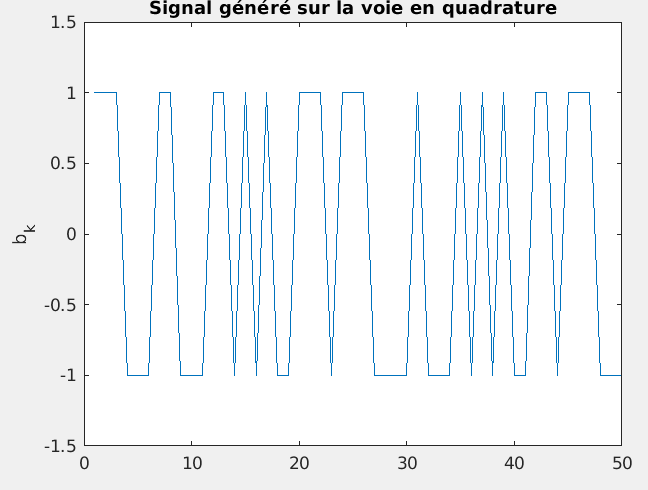
\includegraphics[width=10cm]{C1quadra.png}	              	 	\caption{Signaux générés sur la voies en quadrature (chaîne équivalente passe-bas). \label{F211}}
	\end{figure}
	\newpage
    \item Estimer par périodogramme puis tracer la densité spectrale de puissance de l'enveloppe complexe associée au signal modulé sur fréquence porteuse. Le tracé observé (forme, position) correspond-il à ce qui est attendu en théorie ? Expliquez votre réponse. On comparera notament ce tracé avec celui obtenu pour la DSP du signal sur fréquence porteuse précédemment.
    
    \par\leavevmode\par
    \setlength\parindent{0.5cm}
    La figure \ref{F22} représente l'estimation de la densité spectrale de puissance de l'enveloppe complexe associée au signal modulé sur fréquence porteuse.
    \begin{figure}[ht!]
    		\centering
		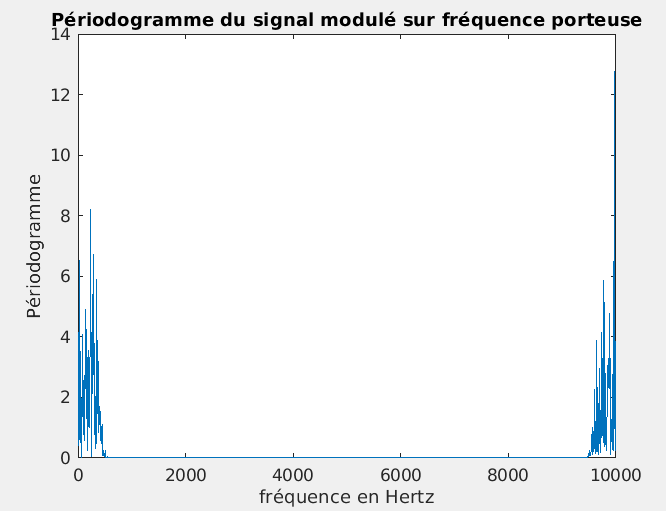
\includegraphics[width=10cm]{C2perio.png}		              	 	\caption{DSP de l'enveloppe complexe associée au signal modulé sur fréquence porteuse. \label{F22}}
	\end{figure}
	
	Cela est cohérant avec ce qui est attendu car on on observe deux pics, un à $0 Hz$ et un à la fréquence $F_e$.
	 
	En comparaison avec la DSP du signal sur fréquence porteuse, ici il n'y a pas de transposition sur fréquence porteuse faite donc les pics sont bien observés à $0$ Hz et $F_e$ Hz et non pas à $f_p$ Hz et $F_e - f_p$ Hz. Cela est dû à la multiplication par la transformée de fourier d'une exponentielle, entraînant une translation de la DSP. 
    \item Implanter la chaine complète sans bruit afin de vérifier que le TEB obtenu est bien nul.
    \par\leavevmode\par
    \setlength\parindent{0.5cm}
    Le TEB obtenu est bien nul.
    
    \item Rajouter le bruit et tracer le taux d'erreur binaire obtenu en fonction du rapport signal à bruit par bit à l'entrée du récepteur ($E_b/N_0$) en décibels. On prendra des valeurs de $\left(E_b/N_0\right)_{dB}$ allant de $0$ à $6$ dB.
    \par\leavevmode\par
    \setlength\parindent{0.5cm}
    La figure \ref{F23} représente le taux d'erreur binaire obtenu en fonction du rapport signal à bruit par bit à l'entrée du récepteur ($E_b/N_0$) en décibels.
    \begin{figure}[ht!]
    		\centering
		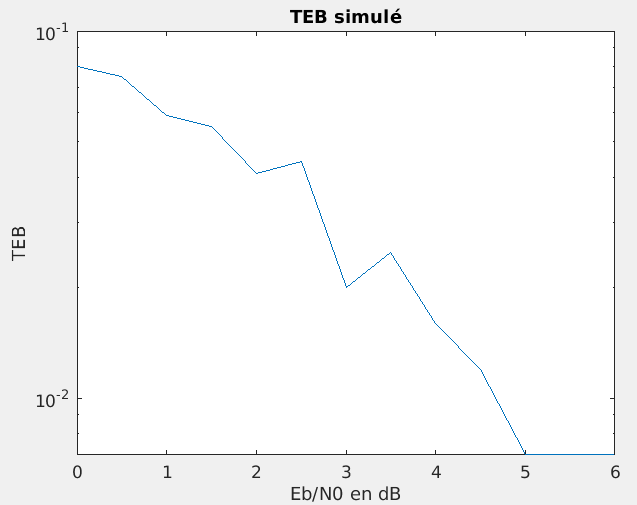
\includegraphics[width=10cm]{C2tebs.png}		              	 	\caption{TEB en fonction de $\left(E_b/N_0\right)_{dB}$ (chaîne passe-bas équivalente). \label{F23}}
	\end{figure}
	\newpage
    \item Tracer les constellations en sortie du mapping et en sortie de l'échantillonneur pour une valeur donnée de $E_b/N_0$.
    \par\leavevmode\par
    \setlength\parindent{0.5cm}
    La figure \ref{F24} représente la constellation en sortie du mapping
    \begin{figure}[ht!]
    		\centering
		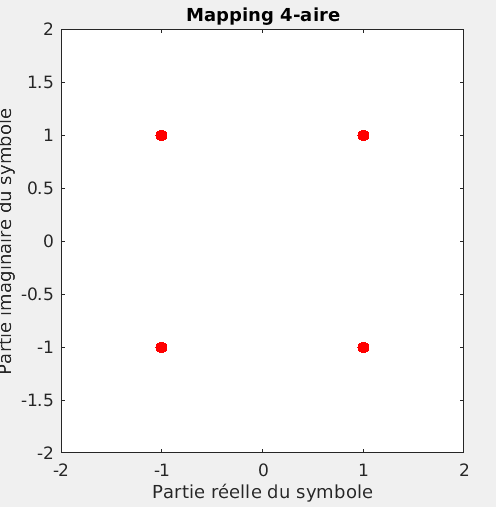
\includegraphics[width=8cm]{C1const.png}		              	 	\caption{Constellation en sortie du mapping. \label{F24}}
	\end{figure}
	\newpage
	 \setlength\parindent{0.5cm}
    La figure \ref{F25} représente la constellation en sortie de l'échantillonneur.
    \begin{figure}[ht!]
    		\centering
		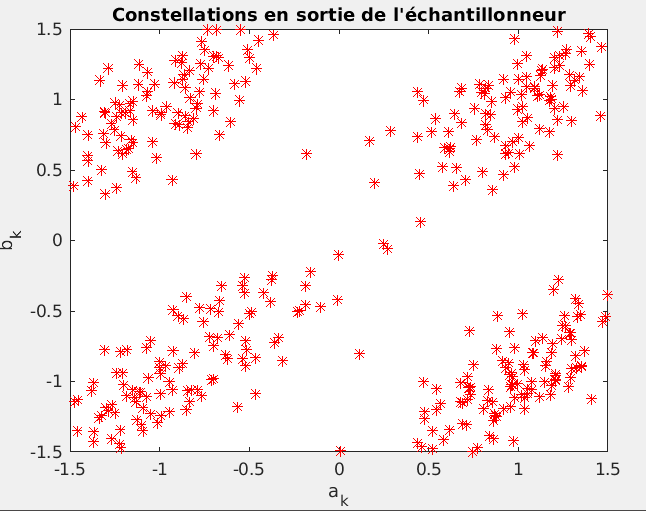
\includegraphics[width=10cm]{C1const1.png}		              	 	\caption{Constellation en sortie de l'échantillonneur. \label{F25}}
	\end{figure}
	
    \item Vérifier que l'on obtient bien le même TEB que celui obtenu avec la chaine simulée sur fréquence porteuse (tracé sur une même figure).
    \par\leavevmode\par
    \setlength\parindent{0.5cm}
    La figure \ref{F26} représente le TEB de la chaîne avec transposition sur fréquence et le TEB de la chaîne équivalente passe-bas. 
    \begin{figure}[ht!]
    		\centering
		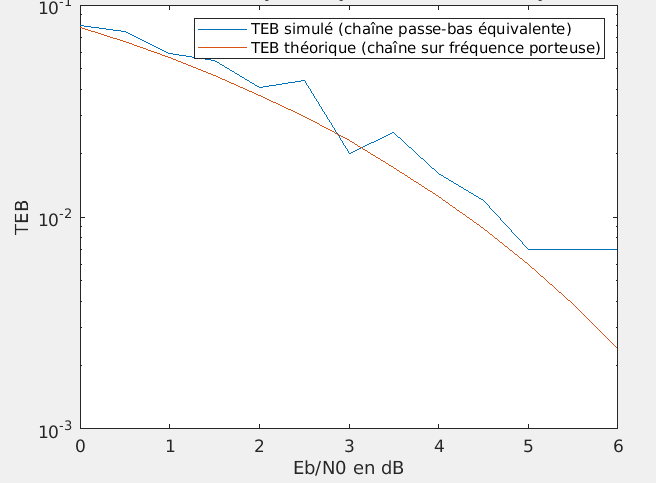
\includegraphics[width=10cm]{C2teb.png}		              	 	\caption{TEB de la chaîne avec transposition sur fréquence et TEB de la chaîne équivalente passe-bas.
		 \label{F26}}
	\end{figure}
	
	On peut conjecturer que la chaîne passe-bande équivalente et la chaîne originelle ont les mêmes TEB. 
\end{enumerate}

%%%%%%%%%%%%%%%%%%%%%%%%%%%%%%%%%%%%%%%%%%%%%%%%%%%%%%%%%%%%%%%%%%
\section{Comparaison de modulations sur fréquence porteuse}
%%%%%%%%%%%%%%%%%%%%%%%%%%%%%%%%%%%%%%%%%%%%%%%%%%%%%%%%%%%%%%%%%%

\subsection{Etude théorique}
On considère les quatre chaines de transmission définies dans le tableau suivant ("SRRCF" signifie "Square Root Raised Cosine Filter" ou filtre en racine de cosinus surélevé en français) :

\begin{table} [H]
\begin{center}
  \begin{tabular}{ |c || c | c | c | c |}
    \hline
    Modulation : & $4$-ASK & QPSK & $8$-PSK & $16$-QAM \\ \hline
    Filtre d'emission : & SRRCF, $\alpha=0,5$ & SRRCF, $\alpha=0,5$ & SRRCF, $\alpha=0,5$ & SRRCF, $\alpha=0,5$ \\ \hline
    Filtre de reception : & SRRCF, $\alpha=0,5$ & SRRCF, $\alpha=0,5$ & SRRCF, $\alpha=0,5$ & SRRCF, $\alpha=0,5$ \\ \hline
    Debit binaire : & $48$ kbps & $48$ kbps & $48$ kbps & $48$ kbps \\ \hline
    TEB :  & $10^{-2}$ & $10^{-2}$ & $10^{-2}$ & $10^{-2}$ \\ \hline
    \hline

  \end{tabular}
\end{center}
% \caption{Comparaison de trois systemes de transmission.}
  \label{table:minus6db}
\end{table}

\begin{enumerate}
    \item Tracer les constellations des quatre modulations considérées.
    
    Pour 16-QAM : 
    \begin{figure}[ht!]
    		\centering
		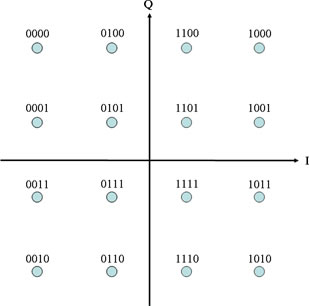
\includegraphics[width=10cm]{C16QAM.jpg}		              	 	\caption{Constellation 16-QAM \label{F31}}
	\end{figure}
	\newpage
	Pour QPSK et 8-PSK : 
	\begin{figure}[ht!]
    		\centering
		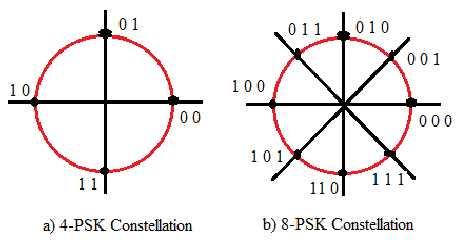
\includegraphics[width=10cm]{CPSK.png}		              	 	\caption{Constellation QPSK \label{F32}}
	\end{figure}
	
	Pour 4-ASK : 
	\begin{figure}[ht!]
    		\centering
		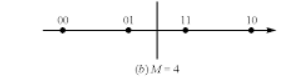
\includegraphics[width=10cm]{C4ASK.png}		              	 	\caption{Constellation 4-ASK \label{F34}}
	\end{figure}
    
    
    \item Déterminer le débit symbole ($R_s$) dans les quatre cas.
    
    $$ R_s = \frac{R_b}{log2(M)}$$
    
    Pour 4-ASK et 4-PSK : 
    $$ R_s = \frac{48}{log2(4)}= 24 \ kbps$$ 
    
    Pour 8-PSK : 
    $$ R_s = \frac{48}{log2(8)} = 16 \ kbps$$ 
    
    Pour 16-QAM: 
    $$ R_s = \frac{48}{log2(16)} = 12 \ kbps$$ 
    
    \item Calculer les efficacités spectrales des quatre transmissions proposées. Quelle est la transmission la plus efficace spectralement ? Qu'est-ce que cela veut dire ?
    \begin{equation*}
    \begin{split}
    \eta & = \frac{R_b}{B} \\
    \eta & = \frac{log2(M)}{k} \\
    \end{split}
    \end{equation*}
     De plus : 
     
    $$ B = (1+\alpha) R_s $$
    
    et : 
    
    $$ B = k R_s $$
    
    D'où : 
    $$ k = 1.5 $$
    
    
    Pour 4-ASK et 4-PSK : 
    $$ \eta \simeq 1.33 \ bits $$ 
    
    Pour 8-PSK : 
    $$ \eta \simeq 2 \ bits $$ 
    
    
    Pour 16-QAM: 
    $$ \eta \simeq 2.67 \ bits $$ 
     
    
     
    \item La figure \ref{comp_TEB} donne les courbes de  TEB obtenus en fonction du rapport signal à bruit par bit à l'entrée du récepteur ($E_b/N_0$) en dB, pour les quatre transmissions considérées réalisées sur canal à bruit additif et Gaussien.
        \begin{itemize}
            \item En déduire les valeurs de $E_b/N_0$ nécessaires pour satisfaire à la spécification du TEB. Quel est le système le plus efficace en terme de puissance ? Justifiez votre réponse.\\
            
            \setlength{\parindent}{0.5cm}
            
            Pour 4-ASK et 16-QAM : $$ \frac{E_b}{N_0} = 8.3 \ dB$$
            
            Pour QPSK : $$ \frac{E_b}{N_0} = 4.4 \ dB$$
            
            Pour 8-PSK : $$ \frac{E_b}{N_0} = 7.5 \ dB$$
            
            Le système le plus efficace en puissance est celui qui nécessite le $\frac{E_b}{N_0}$ le plus faible pour atteindre le TEB fixé. Ici, c'est donc le système utilisant QPSK qui est le plus efficace en puissance. 
            
            \item La chaine de transmission utilisant la modulation $4$-ASK et la chaine de transmission utilisant la modulation $16$-QAM présentent le même taux d'erreur binaire. Qu'est-ce-qui pourrait justifier le choix de l'une ou l'autre ? \\
            
            \setlength{\parindent}{0.5cm}
            Sachant que ces deux chaînes présentent le même taux d'erreur binaire, on choisirait tout de même plutôt la chaîne de modulation $16$-QAM, car elle possède une meilleure efficacité spectrale. 
            
        \end{itemize}
    \item Si on souhaitait réaliser la transmission à travers un canal de propagation supposé à bruit additif blanc et Gaussien (AWGN) de bande passante $20$ kHz, serait-il possible de réaliser chaque transmission proposée en trouvant, au niveau du récepteur, un instant optimal d'échantillonnage sans interférence entre symboles ? Expliquez votre réponse.\\
            
            \setlength{\parindent}{0.5cm}
            On considère ici un canal de type passe-bande (transmission sur fréquence porteuse). 
            
            Afin de respecter le critère de Nyquist, il faut que :
            $$ (1+\alpha) R_s \leq 20000 \ Hz $$
            $$ R_s \leqslant 1333 \ bauds $$
\end{enumerate}

 \begin{figure}[ht!]
    \centering
    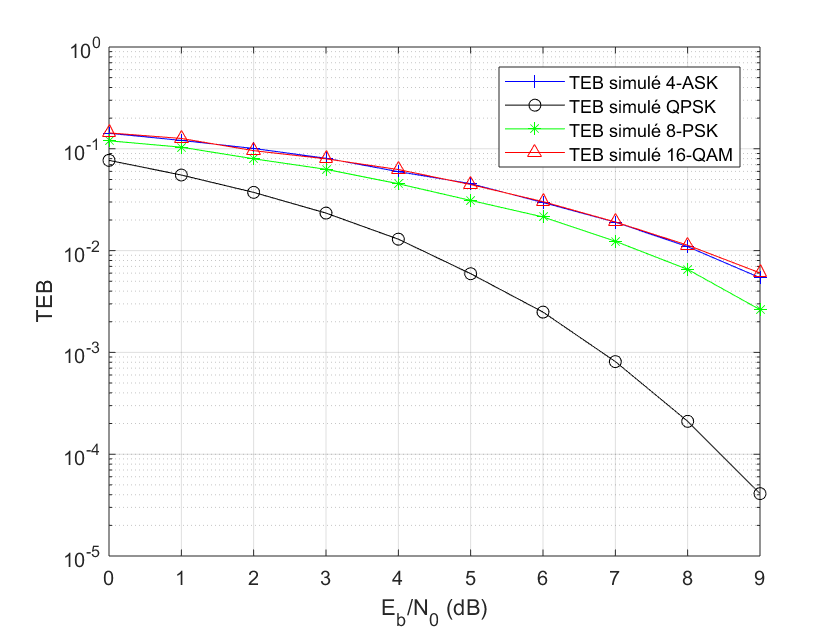
\includegraphics[width=12cm]{Comp_TEB.png}
    \caption{Comparaison des TEB pour les modulations ASK, PSK et QAM}
    \label{comp_TEB}
 \end{figure}

\subsection{Implantation sous Matlab}
Il s'agira d'implanter, d'analyser et de comparer les chaines passe-bas équivalentes associées aux chaines de transmissions proposées dans l'étude théorique.
Pour cela :
\subsubsection{Etude de chaque chaine de transmission}
\begin{enumerate}
    \item Implanter la chaine complète sans bruit afin de vérifier que le TEB obtenu est bien nul. On pourra utiliser les fonctions Matlab \emph{pskmod.m}, \emph{pskdemod.m }et \emph{qammod.m}, \emph{qamdemod.m} pour réaliser les mapping/demapping et prises de décision.
    \item Rajouter le bruit et :
        \begin{itemize}
            \item Tracer les constellations en sortie du mapping et en sortie de l'échantillonneur pour différentes valeurs de $E_b/N_0$, en expliquant les différences observées. \\
            
            La génération de bruit entraîne des erreurs sur la restitution des symboles complexes $d_k$. 
     \begin{figure}[ht!]
    \centering
    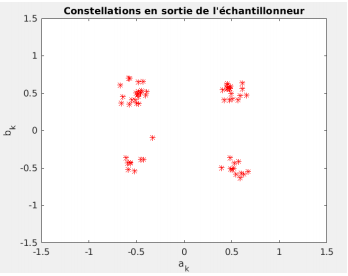
\includegraphics[width=12cm]{C3QPSKconstech.png}
    \caption{Constellation en sortie de l'échantillonneur (QPSK).}
    \label{C35}
 \end{figure}
 
 \begin{figure}[ht!]
    \centering
    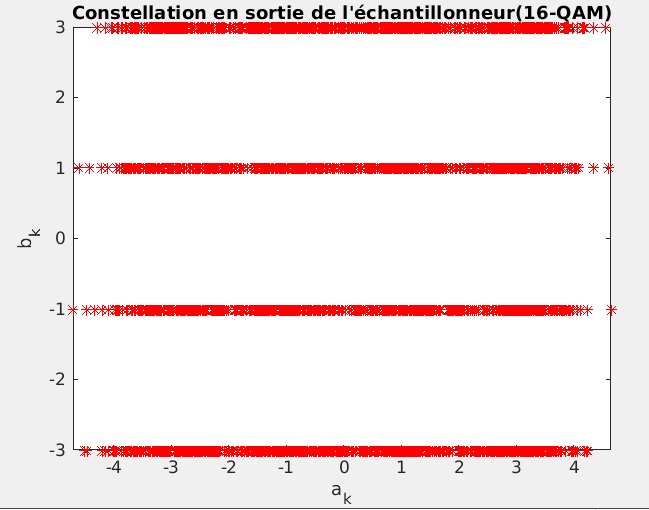
\includegraphics[width=12cm]{C316QAMconstech.png}
    \caption{Constellation en sortie de l'échantillonneur (16-QAM).}
    \label{C35}
 \end{figure}
 
 \begin{figure}[ht!]
    \centering
    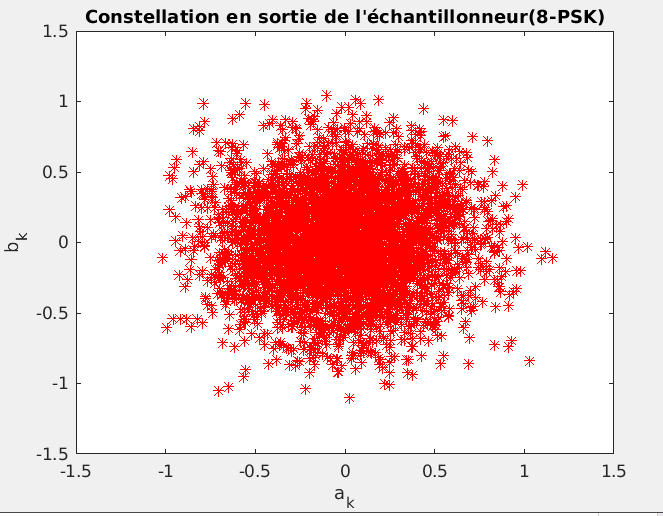
\includegraphics[width=12cm]{C38PSKconstech.png}
    \caption{Constellation en sortie de l'échantillonneur (8-PSK).}
    \label{C35}
 \end{figure}*
 
            \clearpage
            \item Tracer le taux d'erreur binaire obtenu en fonction du rapport signal à bruit par bit à l'entrée du récepteur ($E_b/N_0$) en décibels. On prendra des valeurs de $\left(E_b/N_0\right)_{dB}$ allant de $0$ à $6$ dB.
            \item Comparer le TEB simulé au TEB théorique de la chaine étudiée (tracé superposés sur une même figure). Ce tracé doit permettre de valider le bon fonctionnement de votre chaine de transmission. Les TEBs théoriques sont donnés dans les planches de cours.
   \begin{figure}[ht!]
    \centering
    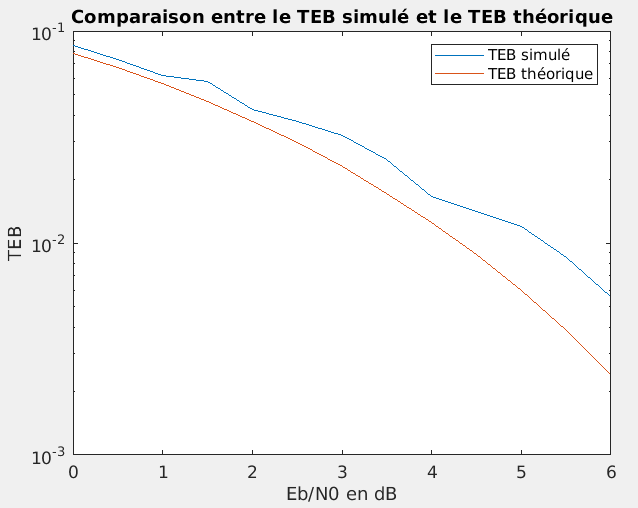
\includegraphics[width=12cm]{C1teb.png}
    \caption{Comparaison des TEB théorique et simulé pour la modulation QPSK.}
    \label{C31}
 \end{figure}
 
 \begin{figure}[ht!]
    \centering
    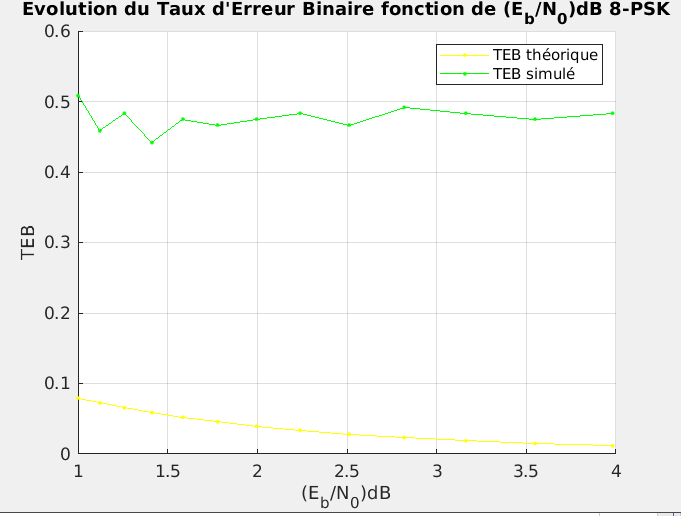
\includegraphics[width=12cm]{C38PSKteb.png}
    \caption{Comparaison des TEB théorique et simulé pour la modulation 8-PSK.}
    \label{C32}
 \end{figure}
 
  \begin{figure}[ht!]
    \centering
    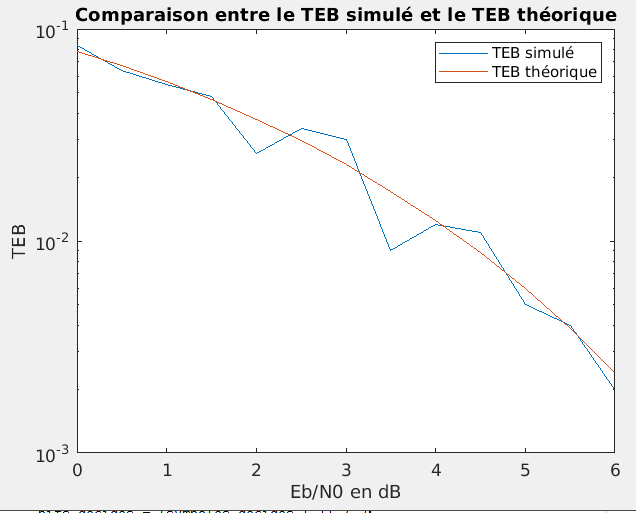
\includegraphics[width=12cm]{C34ASKteb.png}
    \caption{Comparaison des TEB théorique et simulé pour la modulation 4-ASK.}
    \label{C33}
 \end{figure}
 
  \begin{figure}[ht!]
    \centering
    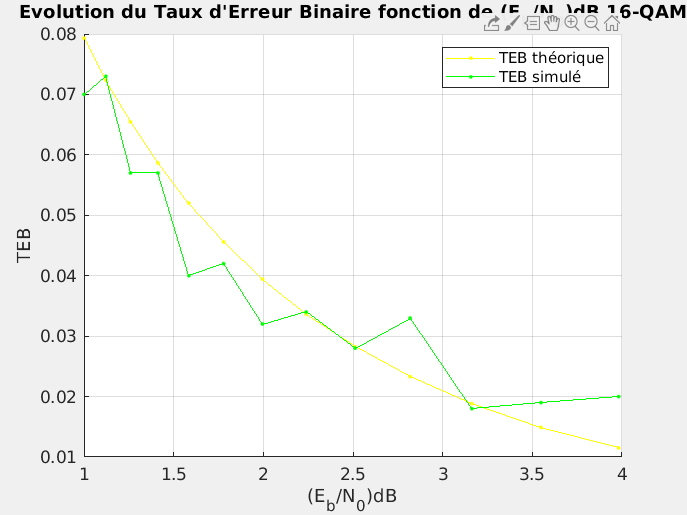
\includegraphics[width=12cm]{C316QAMteb.png}
    \caption{Comparaison des TEB théorique et simulé pour la modulation 16-QAM.}
    \label{C34}
 \end{figure}
            
        \end{itemize}
\end{enumerate}

\clearpage
\subsubsection{Comparaison des chaines de transmission}
\begin{enumerate}
    \item En utilisant les tracés obtenus pour leurs TEBs, comparer et classer les différentes chaines de transmission en en termes d'efficacité en puissance (en expliquant votre raisonnement).
    
    \setlength\parindent{0.5cm}
    L'efficacité en puissance est en lien avec le SNR par bit obtenu à l'entrée du récepteur pour atteindre le TEB souhaité. 
    
    Le système le plus efficace en puissance est celui qui nécessite le $\frac{E_b}{N_0}$ le plus faible pour atteindre le TEB fixé. Ainsi on fixe un TEB (ici $10^{-2}$) et on sélectionne la modulation qui minimise le rapport $(\frac{E_b}{N_0})_{dB}$ correspondant. 
    
    Ici, on observe que le système utilisant QPSK est celui qui est le plus efficace en puissance, suivi par celui utilisant $8$-PSK, puis en dernier celui utilisant $4$-ASK ou $16$-QAM. 
    \item Pour un même débit binaire, tracer les densités spectrales de puissance des signaux émis dans les différentes chaines de transmission étudiées afin de les comparer en termes d'efficacité spectrale et de les classer (en expliquant votre raisonnement).\\
    
    \begin{figure}[ht!]
    \centering
    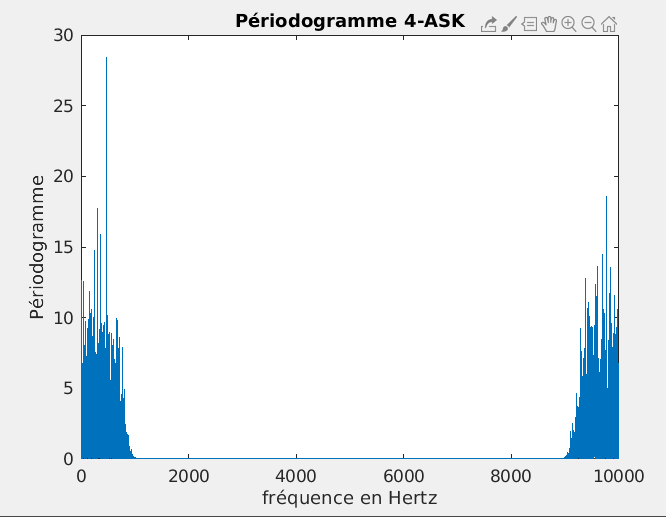
\includegraphics[width=12cm]{C34ASKperio.png}
    \caption{Peridodogramme pour la modulation 4-ASK.}
    \label{C35}
 \end{figure}
 
 \begin{figure}[ht!]
    \centering
    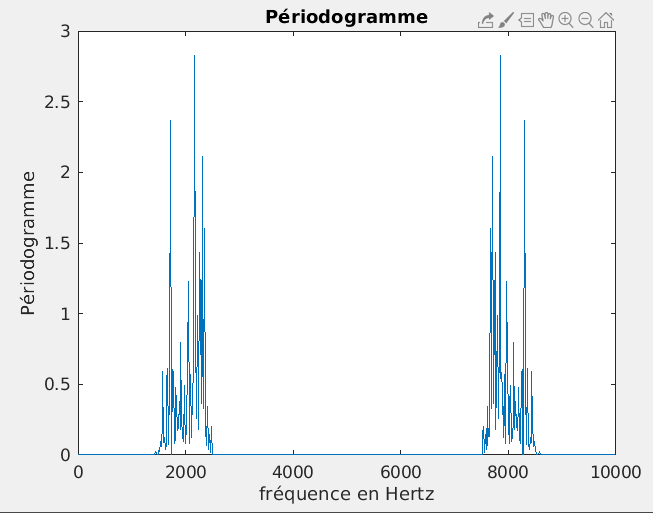
\includegraphics[width=12cm]{C3QPSKperio.png}
    \caption{Peridodogramme pour la modulation QPSK.}
    \label{C35}
 \end{figure}
   
\newpage
    \setlength\parindent{0.5cm}
    L'efficacité spectrale repose sur la largeur de la bande B nécessaire pour transmettre le débit $R_b$ souhaité. Pour un débit binaire donné, plus cette largeur est faible, plus le système est efficace en termes de fréquences.
    On remarque que plus le nombre de symboles possibles est élevé, plus la bande en question est faible. C'est alors que la modulation $16$-QAM est la plus efficace en termes de fréquences, suivie par les modulations $8$-PSK et $4$-ASK/QPSK. 
\end{enumerate}

\section{Conclusion}

A l'issue de cette étude, on peut en conclure que la chaîne  avec transposition sur fréquence porteuse et la chaîne passe-bas équivalente peuvent être confondues en ce qui concerne l'étude menée. 

Sachant que l'efficacité spectrale est proportionnelle au  nombre de symboles possibles (et dépend du filtre de mise en forme), la modulation 16-QAM permet d'avoir la meilleure efficacité spectrale. 

De plus, la modulation QPSK permet d'avoir la meilleure efficacité en puissance. 

Remarquons qu'avec ces modulations-ci , il n'est pas possible de combiner meilleure efficacité spectrale et meilleure efficacité en puissance. 

Et ensuite, il est nécessaire d'imposer le bon débit binaire afin de garantir le respect des conditions de Nyquist. 




\end{document}
